\documentclass[a4paper,11pt,french]{book}
\usepackage[utf8]{inputenc}

\usepackage[T1]{fontenc}
\usepackage[francais]{babel} 
\usepackage[top=2cm, bottom=2cm, left=2cm, right=2cm, includeheadfoot]{geometry} %pour les marges
\usepackage{lmodern}
\usepackage{pict2e}
\usepackage{tikz}	
%\usepackage{tikz-uml}
\usepackage{fancyhdr} % Required for custom headers
\usepackage{lastpage} % Required to determine the last page for the footer
\usepackage{extramarks} % Required for headers and footers
\usepackage{graphicx} % Required to insert images
\usepackage{tabularx, longtable}
\usepackage{color, colortbl}
\usepackage{lscape}
\usepackage[hidelinks]{hyperref}
\usepackage{longtable}
\usepackage{multirow}
\usepackage{rotating}
%\usepackage{pgfgantt}
%\usepackage{gensymb}
\usepackage[toc,page]{appendix} 
\usepackage{pgfplots}
\usepackage{eurosym}
\usepackage{rotating}
\usepackage{array}
\usepgflibrary{arrows} % for pgf-umlsd

\usetikzlibrary{trees,shapes.geometric,arrows,decorations.pathmorphing,backgrounds,fit,positioning,shapes.symbols,chains	}
 \tikzset{
    %Define standard arrow tip
    >=stealth',
    %Define style for boxes
    punkt/.style={
           rectangle, dashed,
           rounded corners,
           draw=black, very thin,
           minimum height=2em,
           minimum width = 2cm,
           text centered},
    square/.style={
           rectangle,
           draw=black, thick,
           minimum height=.5cm,
           minimum width = 1cm,
           text centered},
    data/.style={
           rectangle,
           draw=black, thick,
           minimum height= 2cm,
           minimum width = 2cm,
           text centered},
    % Define arrow style
    pil/.style={
           ->,
           thick,
           shorten <=1pt,
           shorten >=1pt,},
    asym/.style={
           <->,
           thin,
           shorten <=1pt,
           shorten >=1pt,
           red!100},
    sym/.style={
           <->,
           thin,
           shorten <=1pt,
           shorten >=1pt,
           blue!100}
}


%\usetikzlibrary{trees,shapes.geometric,arrows,decorations.pathmorphing,backgrounds,fit,positioning,shapes.symbols,chains	}

\linespread{1.1} % Line spacing

% Set up the header and footer
\pagestyle{fancy}
\lhead{\textbf{\hmwkClass -- \hmwkSubject \\ \hmwkTitle \\ \hmwkDocName}} % Top left header
\rhead{
\includegraphics[width=10em]{logo_univ.png}}
\lfoot{\lastxmark} % Bottom left footer
\cfoot{} % Bottom center footer
\rfoot{Page\ \thepage\ } % Bottom right footer
\renewcommand\headrulewidth{0.4pt} % Size of the header rule
\renewcommand\footrulewidth{0.4pt} % Size of the footer rule

\setlength{\headheight}{40pt}

\newcommand{\hmwkTitle}{Chat sécurisé} % Assignment title
\newcommand{\hmwkClass}{Master 1 SSI } % Course/class
\newcommand{\hmwkAuthorName}{Charles Ango, Ismael Kabore,  Julien Legras, Yves Nouafo, Jean-Baptiste Souchal} % Your name
\newcommand{\hmwkSubject}{Conduite de projet} % Subject
\newcommand{\hmwkDocName}{Rapport de projet} % Document name

\newcommand{\version}{1.2} % Document version
\newcommand{\docDate}{24 mai 2013} % Document date
\newcommand{\checked}{Julien Legras} % Checker name
\newcommand{\approved}{} % Approver name

\definecolor{gris}{rgb}{0.95, 0.95, 0.95}

\title{
\vspace{2in}
\textmd{\textbf{\hmwkClass :\ \hmwkTitle}}\\
\normalsize\vspace{0.1in}\small{Due\ on\ \hmwkDueDate}\\
\vspace{0.1in}\large{\textit{\hmwkClassInstructor\ \hmwkClassTime}}
\vspace{3in}
}

\author{\hmwkAuthorName}
\date{} % Insert date here if you want it to appear below your name

\makeatletter
\def\chapter{\if@openright\cleardoublepage\else\clearpage\fi
  \global\@topnum\z@
  \@afterindentfalse
  \secdef\@chapter\@schapter}
\makeatother


\begin{document}
\pagestyle{empty}

\vspace*{1cm}
\begin{center}

\includegraphics[width=20em]{logo_univ.png}
\end{center}
\vspace*{2cm}
\begin{center}\textbf{\huge{Master 1 Sécurité des systèmes informatiques}}\end{center}
\vspace*{1cm}
\begin{center}
\textbf{\Huge{\hmwkDocName}: \hmwkTitle}
\end{center}

\vspace*{3cm}
	

\fcolorbox{black}{gris}{
\begin{minipage}{15cm}
\begin{tabularx}{10cm}{lXp{8cm}}
	& & \\
	\bfseries{Rédigé par} & & \hmwkAuthorName \\
	& & \\
	\bfseries{Relu par} & & \checked \\
	& & \\
	\bfseries{À l'attention de} & & Magali Bardet\\
	& & \\
	\bfseries{Date de rendu} & & \docDate\\
	& & \\
\end{tabularx}
\end{minipage}
}

\newpage


%%%%%%%%%%%%%%%%%%%%%%%%%%%%%%%%%%%%%%%%%%%%
% Introduction
% JB
%%%%%%%%%%%%%%%%%%%%%%%%%%%%%%%%%%%%%%%%%%%%
\frontmatter
\pagestyle{fancy}
\large
\chapter{Introduction}

Les outils de messagerie instantanée sont de nos jours largement utilisés par les particuliers et entreprises. Ces communications donnent 
parfois lieu à des échanges de données confidentielles. Or, la sécurité des données et l'authentification des utilisateurs n'y sont généralement pas assurées. Il est donc important 
d'avoir à disposition des outils permettant d'assurer la confidentialité d'une 
communication. C'est donc dans le cadre de notre projet annuel de première année 
de master en sécurité des systèmes informatiques que nous avons étudié les protocoles cryptographiques permettant à plusieurs utilisateurs de s'authentifier et de communiquer de manière sécurisée à travers un
outil de messagerie instantanée assurant la confidentialité et l'intégrité 
des données échangées.\\

La couche de sécurité mise en place sur un outil de 
messagerie instantanée va permettre de dialoguer avec des utilisateurs 
authentifiés, d'assurer l'intégrité des 
messages reçus, c'est-à-dire que le message n'a pas été modifié entre deux 
interlocuteurs puis une confidentialité assurée des contenus échangés grâce à 
des outils cryptographiques forts mis en place empêchant toute intelligibilité des 
données transitant entre utilisateurs pour quelqu'un de non autorisé.\\

Dans un premier temps nous allons faire une présentation plus détaillée du sujet 
en analysant les besoins du client puis nous présenterons les solutions proposées. Nous détaillerons ensuite les résultats obtenus après 
l'implémentation des solutions proposées en amont et leur pertinence par rapport aux besoins du client.
Finalement un manuel d'utilisation viendra compléter ce rapport afin d'assurer une 
bonne prise en main de l'outil de messagerie instantanée par le client.

%La table des matières
\tableofcontents



\newpage
\mainmatter
%%%%%%%%%%%%%%%%%%%%%%%%%%%%%%%%%%%%%%%%%%%%
% PRÉSENTATION DU PROJET 
% Yves & Julien
%%%%%%%%%%%%%%%%%%%%%%%%%%%%%%%%%%%%%%%%%%%%
\chapter{Présentation du projet}
Dans le cadre de notre projet, il nous à été demandé de réaliser un système de bavardage sécurisé. Pour le mener à bien, le travail à été découpé en deux grandes phases qui sont l'analyse des besoins du client et les solutions proposées.

\section{Besoins du client}
Les fonctionnalités du logiciel sont les points indispensables, nécessaires et imposés par le client. Dans notre sujet, on le résume de la manière suivante:\\ 

\textbf{\'Etudier les protocoles cryptographiques permettant à plusieurs utilisateurs de s’authentifier et de communiquer de manière sécurisée à travers un outil de messagerie instantanée répondant au standards IRC.}\\

\`A la fin du développement, l'outil de messagerie instantanée devra répondre aux besoins du client, garantir que les messages soient échangés entre utilisateurs, prouver la mise en place du système de sécurité ainsi que les protocoles déployés pour parvenir à un système de bavardage sûr.

\section{Solutions proposées}
\`A l'issue de l'analyse des besoins du client, il a été convenu de traiter sa demande en décomposant la réalisation du logiciel en trois phases de développement :
\begin{itemize}
\item \textbf{Phase 1:} Mise en place du système de bavardage modèle client-serveur;
\item \textbf{Phase 2:} Installation d'une PKI (infrastructure à clés publiques);
\item \textbf{Phase 3:} Mise en place d'une couche sécurisée pour permettre une communication chiffrée, authentifiée et d'en garantir l'intégrité.
\end{itemize}
\vspace{.5cm}

\subsection{Structure du logiciel}
Le logiciel est conçu et pensé de manière modulable de tel sorte que chaque partie puisse \^etre utilisée de manière indépendante. Son architecture se présente ainsi:\\

\begin{center}
\begin{tikzpicture}[node distance=-.01cm,font=\tiny,scale=1.8,every node/.style={transform shape}]
		\node[square, text width=1.5cm, fill=white!100] (appclient) at (0,0) {Application client};
		\node[square, text width=2cm, fill=white!100] (modclientsec) at (4,0) {Module client sécurisé};
		\begin{pgfonlayer}{background} 
		\node[punkt, fit=(appclient)(modclientsec), fill=blue!20] (groupclient) {};
		\end{pgfonlayer}
		
		\node[square, text width=1cm, fill=white!100] (PKI) at (2.5,-1.5) {PKI};
		\node[square, text width=1cm, fill=white!100] (serveur) at (0,-2.5) {Serveur};
		\node[square, text width=1.5cm, fill=white!100] (serveurs) at (4,-2.5) {Serveur sécurisé};
		\begin{pgfonlayer}{background} 
		\node[punkt, fit=(PKI)(serveur)(serveurs), fill=green!20] (groupserveur) {};
		\end{pgfonlayer}

		\node[text width=.7cm] (imgbd1) at (0,-4) {
\includegraphics[height=3em]{computer-database.png}};
		\node[square, text width=.5cm, below=of imgbd1, fill=white!100] (bd1){BDD};
		\node[text width=.7cm] (imgfichiers) at (2.5,-4) {
\includegraphics[height=3em]{computer-database.png}};
		\node[square, text width=.7cm, below=of imgfichiers, fill=white!100] (fichiers){BDD};
		\node[text width=.7cm] (imgbd2) at (4,-4) {
\includegraphics[height=3em]{computer-database.png}};
		\node[square, text width=.5cm, below=of imgbd2, fill=white!100] (bd2){BDD};

		\begin{pgfonlayer}{background} 
		\node[punkt, fit=(imgbd1) (bd1) (imgbd2) (bd2) (imgfichiers) (fichiers), fill=orange!20] (stock) {};
		\end{pgfonlayer}


		\draw (appclient.east) edge[<->] (modclientsec.west);
		\draw (appclient.south) edge[<->] (serveur.north);
		\draw (modclientsec.south west) edge[<->] (PKI.north);
		\draw (modclientsec.south) edge[<->] (serveurs.north);
		
		\draw (serveur.south) edge[<->] (imgbd1.north);
		\draw (serveurs.south) edge[<->] (imgbd2.north);
		\draw (PKI.south) edge[<->] (imgfichiers.north);
		\draw (PKI.south east) edge[<->] (serveurs.north);
		
		\draw (PKI.west) edge[->, loop left = 90] (PKI.west);

		\begin{pgfonlayer}{background} 
		\node[minimum width=2.5cm, minimum height=6.3cm,rectangle, draw=black!60!green, very thick, fit=(appclient) (serveur) (imgbd1) (bd1)] (groupeclassic) {};
		\node[minimum width=4cm, minimum height=6.3cm,rectangle, draw=black!30!red, very thick, fit=(modclientsec) (PKI) (serveurs) (imgbd2) (bd2) (imgfichiers) (fichiers)] (groupesec) {};
		\end{pgfonlayer}
		
		\node[below=of groupeclassic, color=black!60!green] (legendgpeclassic) {Chat classique};		
		\node[below=of groupesec, color=black!30!red] (legendgpesec) {Partie sécurisée};

		\node[right=of modclientsec, minimum width=3cm] (lgdappcl) {Application client};
		
		\node[right=of groupserveur, minimum width=3cm] (lgsrv) {Serveurs};
		
		\node[right=of stock, minimum width=4cm, anchor=west] (lgbdd) {Bases de données};

		\end{tikzpicture}
		\end{center} 
		\vspace{.3cm}
		
Sur le schéma précédent on voit bien la séparation de la partie couche classique de la partie couche sécurisée, mais aussi les différentes couches qui interviennent dans le développement du logiciel. Ces couches sont la partie client, la partie serveurs et la partie base de données.\\

La partie Application client comporte deux modules qui sont l'application client et le module client sécurisé. L'application client permet à l'utilisateur de pouvoir communiquer avec d'autres utilisateurs de manière classique. Autrement dit, chaque message pourra être lu par tout utilisateur présent dans un salon.\\Quant au module client sécurisé, il permet d'établir une communication sécurisée entre plusieurs utilisateurs. Une communication sécurisée masque le message à tout utilisateur n'étant pas destinataire du message en question. \\Cette partie implémente les principales fonctionnalités suivantes:
\begin{itemize}
\item création d’un compte sécurisé;
\item envoi de message sur salon privé;
\item envoi de message sur salon général;
\item rejoindre un serveur de chat sans authentification;
\item quitter un serveur de chat;
\item envoi d’un message privé non sécurisé;
\item créer un salon privé;
\item joindre un salon privé;
\item fermeture d’un salon privé.
\end{itemize}
\vspace{.6cm}

La partie serveurs est décomposée en trois éléments qui sont le serveur, le serveur sécurisé et la PKI. Chacun de ces éléments ont un rôle bien défini. \\Le rôle du serveur est de distribuer les messages aux destinataires.\\Le rôle du serveur sécurisé est d'authentifier les utilisateurs sécurisés et de distribuer les clés symétriques permettant le chiffrement, le déchiffrement et l'intégrité des messages entre utilisateurs sécurisés.\\La PKI est une autorité de confiance qui permet d'établir l'authenticité d'un utilisateur sécurisé. Nous avons opté pour une PKI clé en main EJBCA qui remplira les fonctionnalités suivantes :
\begin{itemize}
\item ajout d'un certificat à un utilisateur;
\item révocation d’un certificat.
\end{itemize}
\vspace{.6cm}

La partie base de données décrit les données manipulées et utiles à l'application. L'application globale en possède trois.\\
La première permet la gestion des utilisateurs non sécurisés. Cette base de données est rattachée au serveur non sécurisé. Elle est non persistante, ce qui veut dire que lors de la fin de l'utilisation du logiciel par un utilisateur, celui-ci ne sera pas conservé en base. Cette base à pour rôle de lister tout utilisateur déjà présent sur le service de chat.\\
La seconde permet la gestion des utilisateurs sécurisés. Contrairement à la première, cette base est persistante, ce qui permet à tout utilisateur sécurisé de réserver son nom et de pouvoir l'utiliser pour les prochaines connections à venir sur le service.\\ La dernière permet le stockage des certificats générés par la PKI. Ces certifcats définissent l'identité d'un utilisateur et sont stockés dans une base de données interne à l'application EJBCA.

\subsection{Détail de la couche sécurisée}
La couche sécurisée contient le module sécurisé, la PKI, le serveur sécurisé et la base de données qui lui est jointe. Cette couche est nécessaire pour échanger et garantir l'échange des messages sécurisés sans que celui-ci ne puisse être lu par un autre utilisateur. Pour mettre en place cette partie, on utilise la bibliothèque OpenSSL pour assurer la création d'un canal de communication sécurisé entre deux utilisateurs sécurisés.\\Comme dit ci-dessus, la PKI, autorité de confiance, permettra de garantir et d'identifier les utilisateurs présents sur le système de chat. On a aussi vu précédemment quel rôle joue le serveur sécurisé. Toute la mise en \oe uvre ainsi décrite permet de garantir un système de chat respectant les normes et les exigences du client. \\

Pour s'assurer que l'application fournie respecte bien les exigences du client, elle implémente des exigences fonctionnelles que l'on peut retrouver dans le {cahier de recette}, où on peut voir les différents tests garantissant la mise en place de la couche sécurisée.

\subsection{Choix des langages}
Le choix des langages pour réaliser le projet sont le C pour la réalisation du serveur non sécurisé et du serveur sécurisé ainsi que des clients, sécurisé et non sécurisés.\\La réalisation de la base de données embarquée s'est faite en sqlite.\\La partie graphique quant à elle a été faite en Vala, car ce langage s'interface avec le C très facilement.\\
Pour la partie sécurisée on a choisi la bibliothèque OpensSSL car elle fourni une bibliothèque riche en fonctions cryptographiques.

\section{Partie technique}

Le résultat a été réparti en trois livraisons dont voici les contenus.

\subsection{Partie non-sécurisée}
La première partie consistait en le développement d'un client et d'un serveur de chat. 
Pour la communication entre les clients et le serveur, une structure C a été mise en place :

\begin{verbatim}
typedef struct {
        int code;
        char sender[MAX_NAME_SIZE];         // MAX_NAME_SIZE = 64
        char content[MAX_MESS_SIZE];        // MAX_MESS_SIZE = 512
        char receiver[MAX_ROOM_NAME_SIZE];  // MAX_ROOM_NAME_SIZE = 64
} message;
\end{verbatim}

Chaque action est représentée par un code (\verb+CONNECT, CREATE_ROOM, MESSAGE...+). Le champ \verb+sender+ représente l'émetteur du message, \verb+receiver+ le destinataire. Enfin le champ \verb+content+ contient le(s) argument(s) associé(s) à l'action souhaitée. Côté client, pour envoyer une telle structure, il suffit d'appeler la fonction \verb+int send_message(const char *mess,+\\ \verb+char **error_mess)+ avec \verb+mess+ de la forme : \verb+"/<ACTION> <ARGS>"+ et \verb+err_mess+ le message d'erreur, si une erreur survient. L'affichage de message reçu se fait à la couche supérieure, dans l'interface graphique ou en lignes de commandes en appelant la fonction \verb+int receive_message(+\\\verb+message *m)+. Ces fonctions se trouvent dans une bibliothèque écrite pour le client (\verb+libclient.a+) afin de les utiliser dans l'interface graphique et en préparation à la surcouche sécurisée de la troisième livraison. 

L'interface du client de chat a été développée en Vala à l'aide de la bibliothèque graphique GTK. La fenêtre a été dessinée à l'aide de Glade qui est un User Interface Designer produisant un fichier \verb+.xml+, ce dernier étant utilisé dans le code Vala.

Côté serveur, les clients sont gérés dans des fils d'exécution séparés. Chaque message reçu est filtré selon son code d'action et le traitement correspondant est effectué. Si la connexion avec un client est perdue, le fil d'exécution s'arrête en déconnectant l'utilisateur.

\subsection{Certification}
La seconde livraison consistait en la mise en place d'une infrastructure à clefs publiques (PKI). Cette infrastructure permet de garantir l'identité d'un utilisateur en lui délivrant un certicat numérique qui permet d'effectuer des opérations cryptographiques. Pour cela nous avons utilisé EJBCA (Enterprise Java Bean Certificate Authority) qui est une application utilisant un serveur JBoss. L'installation s'est faite en quelques étapes :

\begin{paragraph}{Récupération de JBoss et d'EJBCA}
\small{
\begin{verbatim}
$ wget http://sourceforge.net/projects/jboss/files/JBoss/JBoss-5.1.0.GA/jboss-5.1.0.GA-jdk6.zip
$ wget http://sourceforge.net/projects/ejbca/files/ejbca4/ejbca_4_0_10/ejbca_4_0_10.zip
$ unzip jboss-5.1.0.GA-jdk6.zip
$ unzip ejbca_4_0_10.zip
\end{verbatim}
}
\end{paragraph}

\begin{paragraph}{Configuration et construction d'EJBCA}
\small{
\begin{verbatim}
$ echo "appserver.home=/home/user/jboss-5.1.0.GA" >> ejbca_4_0_10/conf/ejbca.properties
$ cd ejbca_4_0_10; ant bootstrap 
\end{verbatim}
}
\end{paragraph}

\begin{paragraph}{Installation et déploiement d'EJBCA}
\small{
\begin{verbatim}
$ /home/user/jboss-5.1.0.GA/bin/run.sh &
$ ant install
$ ant deploy
\end{verbatim}
}
\end{paragraph}
\newpage

Pour la configuration des autorités de certification et des différents profils, EJBCA met à disposition une interface web. Il faut tout d'abord récupérer le certificat administrateur qui a été généré lors de l'installation se trouvant dans \verb+/home/user/ejbca_4_0_10/p12/superadmin.p12+ puis de l'ajouter dans les certificats du navigateur comme suit (Firefox) :

\begin{center}
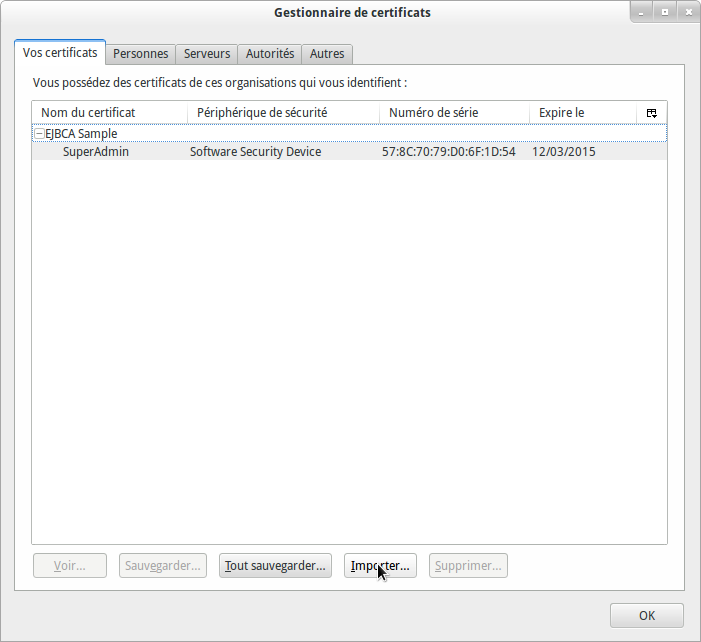
\includegraphics[width=30em]{import_superadmin.png}
\end{center}

On peut alors accéder à la partie administration à partir de l'adresse:

\verb+https://inf-srv-securechat:8443/ejbca/adminweb/index.jsp+
\newpage
La page obtenue est la suivante :
\begin{center}
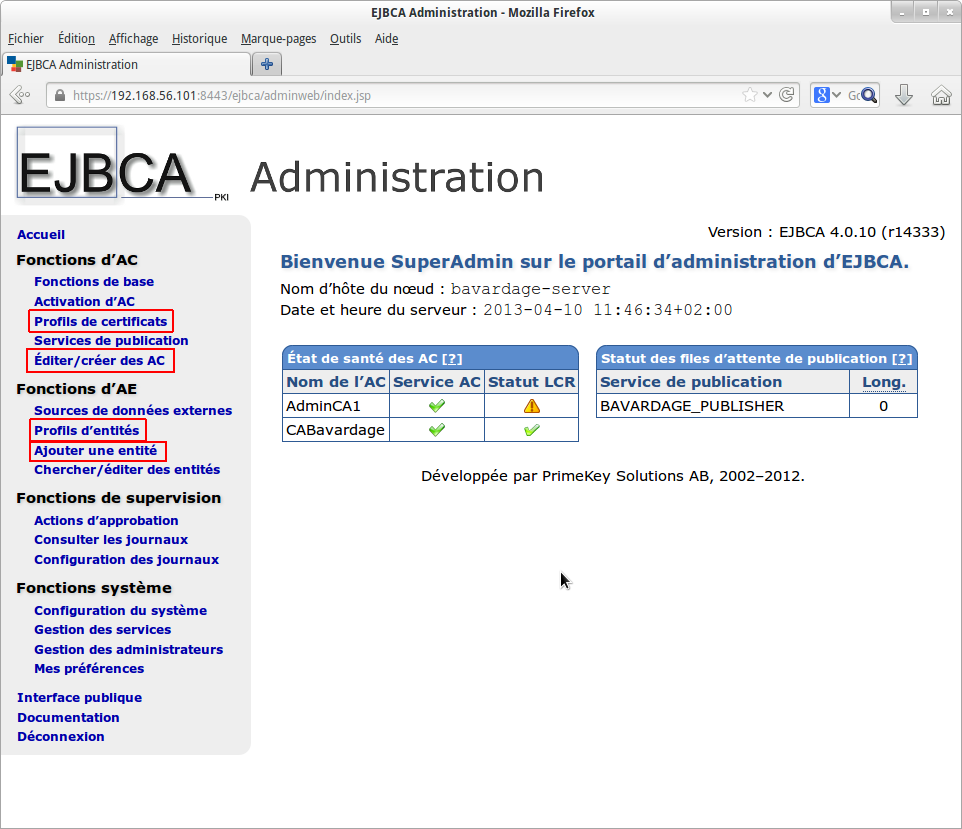
\includegraphics[width=40em]{admin_ejbca.png}
\end{center}

Les parties importantes ont été entourées en rouge et voici leurs descriptions.\\

Les profils contiennent les informations nécessaires et utiles qui permettent de générer les certificats. Comme on peut voir sur le schéma précédent, il en existe deux sortes.
\begin{paragraph}{Profils de certificats}
C'est dans cette section que l'on crée les différents profils de certificats :
\begin{itemize}
\item \verb+BAVARDAGESERVER+ : profil pour le serveur sécurisé ;
\item \verb+BAVARDAGEUSER+ : profil pour les utilisateurs sécurisés.
\end{itemize}

\begin{paragraph}{Profils d'entités}
Chaque type d'entité a un profil associé:
\begin{itemize}
\item \verb+BAVARDAGE_SERVER+ : profil pour le serveur sécurisé ;
\item \verb+BAVARDAGE_USER+ : profil pour les utilisateurs sécurisés.
\end{itemize}
On utilise deux profils d'entités différents car les rôles de chacun sont différents. Le premier pour déterminer l'entité du server et le second l'entité de l'utilisateur.
\end{paragraph}
\end{paragraph}
\\
Ces profils sont décrits en détail dans le document annexe : Politique de certification


\begin{paragraph}{Éditer/créer des AC}
Une AC (autorité de certification) est une entité dont la mission est de vérifier les données du demandeur de certificat, de signer et de maintenir une liste des certificats et une liste des révocations. Sur la capture d'écran ci-dessus, on voit la liste des AC contenant celle relative à notre projet : \verb+CABavardage+
\end{paragraph}


\begin{paragraph}{Ajouter une entité}
Lorsqu'un utilisateur désire obtenir un certificat, un administrateur doit au préalable lui créer une entité associée. Il pourra ensuite récupérer son certificat pour sa clef RSA.
\end{paragraph}


\subsection{Partie sécurisée}
La troisième livraison consistait en la surcouche sécurisée du client de chat et un serveur « sécurisé » dont le rôle est de gérer les utilisateurs sécurisés et la sécurité des messages.

Nous avons choisi tout d'abord d'ouvrir une connexion SSL entre le client sécurisé et le serveur sécurisé grâce aux fonctions d'OpenSSL. Ensuite, nous avons crée des codes d'actions spécifiques à l'utilisation sécurisée du chat comme \verb+CONNECT_SEC, CREATE_ROOM_SEC+... La gestion des clients dans le serveur sécurisé est similaire au serveur classique avec un fil d'exécution par client et une socket SSL.

Côté client, la surcouche sécurisée se base sur la bibliothèque du client classique et utilise la même logique. Ainsi nous avons deux fonctions principales : 
\begin{itemize}
\item \verb+int send_message_sec (const char *mess, char **err_mess)+
\item \verb+int receive_message_sec (message *m)+
\end{itemize}

On rajoute également des fonctions de chiffrement/déchiffrement de messages :
\small{
\begin{itemize}
\item \verb+char *aes_encrypt (unsigned char *key, unsigned char *iv, char *plaintext, int *len)+

\item \verb+char *aes_decrypt (unsigned char *key, unsigned char *iv, char *ciphertext, int *len)+
\end{itemize}
}
\large
Pour le chiffrement et le déchiffrement nous utilisons une fonction \\
 \verb+char *gen_keyiv(key_iv keyiv, unsigned char *key_data, int key_data_len)+ 
 qui génère la clé et l'IV (valeur d'initialisation). C'est cette paire (clé, iv) qui est utilisée par les fonctions \verb+aes_encrypt+ et \verb+aes_decrypt+ pour chiffrer et déchiffrer les messages.

Comme les noms des fonctions l'indiquent, nous utilisons AES-256-CBC pour chiffrer les messages envoyés (champ \verb+content+). AES est un chiffrement par bloc qui supporte des clés et des blocs de 128, 192 et 256 bits. Le mode de chiffrement CBC consiste à diviser les données en plusieurs blocs de même taille et à les chiffrer de manière chaînée (le résultat précédent est utilisé lors du chiffrement suivant). L'IV est utilisée pour le chiffrement du premier bloc. Avec le mode CBC l'IV est unique et aléatoire, ce qui rend la clé réutilisable sans risque, et il n'y a pas de risque de répétition de bloc. Nous avons choisi AES-256-CBC pour avoir une plus grande taille des clés et la sécurité qu'offre le mode de chiffrement CBC. 


\section{Problèmes rencontrés}
Nous avons rencontré un problème pour la livraison du sprint 2. En effet, nous devions configurer un serveur, ce que nous avions fait dans une machine virtuelle. Cependant, le format de livraison utilisé jusqu'alors n'était plus utilisable car la machine faisait plusieurs giga octets de données. Nous avons alors convenu avec Mme Bardet de livrer sur une clef USB dans un premier temps et de configurer une machine mise à disposition par Mr Macadré en début du sprint 3.

Pour le sprint 3, nous avons également eu des problèmes au niveau de l'apprentissage d'OpenSSL. En effet, nous n'avions aucune expérience avec cette bibliothèque et les exemples sont nombreux mais très différents. Finalement, Mme Bardet nous a conseillé un très bon ouvrage : Network Security with OpenSSL.



\newpage
%%%%%%%%%%%%%%%%%%%%%%%%%%%%%%%%%%%%%%%%%%%%
% MANUEL D'UTILISATION 
% Charles & Ismaël
%%%%%%%%%%%%%%%%%%%%%%%%%%%%%%%%%%%%%%%%%%%%
\chapter{Manuel d'utilisation}
\section{Récupération du projet}
 Les sources du projet sont disponibles sur un dépôt git. Elles peuvent être récupérées en ligne de commande ou en ligne. 
 
 \subsection{En ligne de commande}
 Placez vous dans un terminal et exécutez la commande suivante :
\begin{verbatim} 
    $ git clone git://github.com/legrajul/bavardage.git 
\end{verbatim}

\subsection{En ligne}
 Une archive contenant le projet peut être téléchargée à l'adresse :
 
\url{https://github.com/legrajul/bavardage/archive/master.zip}

\section{Compilation}
\subsection{Dépendances Ubuntu}
Pour la compilation du projet il faut d'abord vérifier si toutes les dépendances sont satisfaites :
\begin{itemize}
\item gcc : permet de compiler le code C.
\item cmake : permet de précompiler un projet pour différentes plateformes et de générer des makefile.
\item valac-0.18 : compilateur Vala qui précompile (dans notre cas) le code source vala en code source C.
\item libgtk-3-dev : bibliothèque multi plateformes pour créer des interfaces graphiques.
\item libgee-dev : bibliothèque de collections fournissant des classes basées sur GObject.
\item libglib2.0-dev : fichiers de développement pour la bibliothèque GLib.
\item libssl-dev : bibliothèque de développement OpenSSL.
\item libsqlite3-dev : bibliothèque de développement SQLite.
\end{itemize}

\subsection{Compilation des sources}

Les commandes suivantes doivent être exécutées dans le dossier racine du projet git bavardage : 
\begin{verbatim}
    $ mkdir src/build 
    $ cd src/build 
    $ cmake .. 
    $ make
\end{verbatim}

\section{Exécution}

\subsection{Demande de certificat}

Pour faire une demande de création de compte sécurisé, l'utilisateur doit envoyer un e-mail à julien.legras@etu.univ-rouen.fr . Il faut renseigner les informations suivantes:
\begin{itemize}
\item les noms et prénoms
\item le pays
\item la ville
\item l'organisation
\item l'adresse mail
\item le département
\end{itemize}

L'utilisateur peut entrer ce qu'il veut dans les différents champs. Seul les éléments entrés par l'administrateur sur EJBCA seront pris en compte.
Après avoir reçu le message de confirmation de compte créé par l'administrateur, il faut générer une clé RSA 2048 avec la commande:

\verb+ $ openssl genrsa -out maclef.pem 2048 -aes256+

Puis on crée la requête:

\verb+ $ openssl req -new -key maclef.pem -out marequete.req+

Pour récupérer son certificat, il faut aller dans la partie publique du site web à l'adresse \url{http://inf-srv-securechat:8080/ejbca/enrol/server.jsp} puis :
\begin{itemize}
\item Entrer les identifiants (login/mot de passe) fournis par l'administrateur;
\item Selectionner le fichier "marequete.req" généré sur votre ordinateur;
\item Valider avec le bouton "OK".
\end{itemize}

\newpage
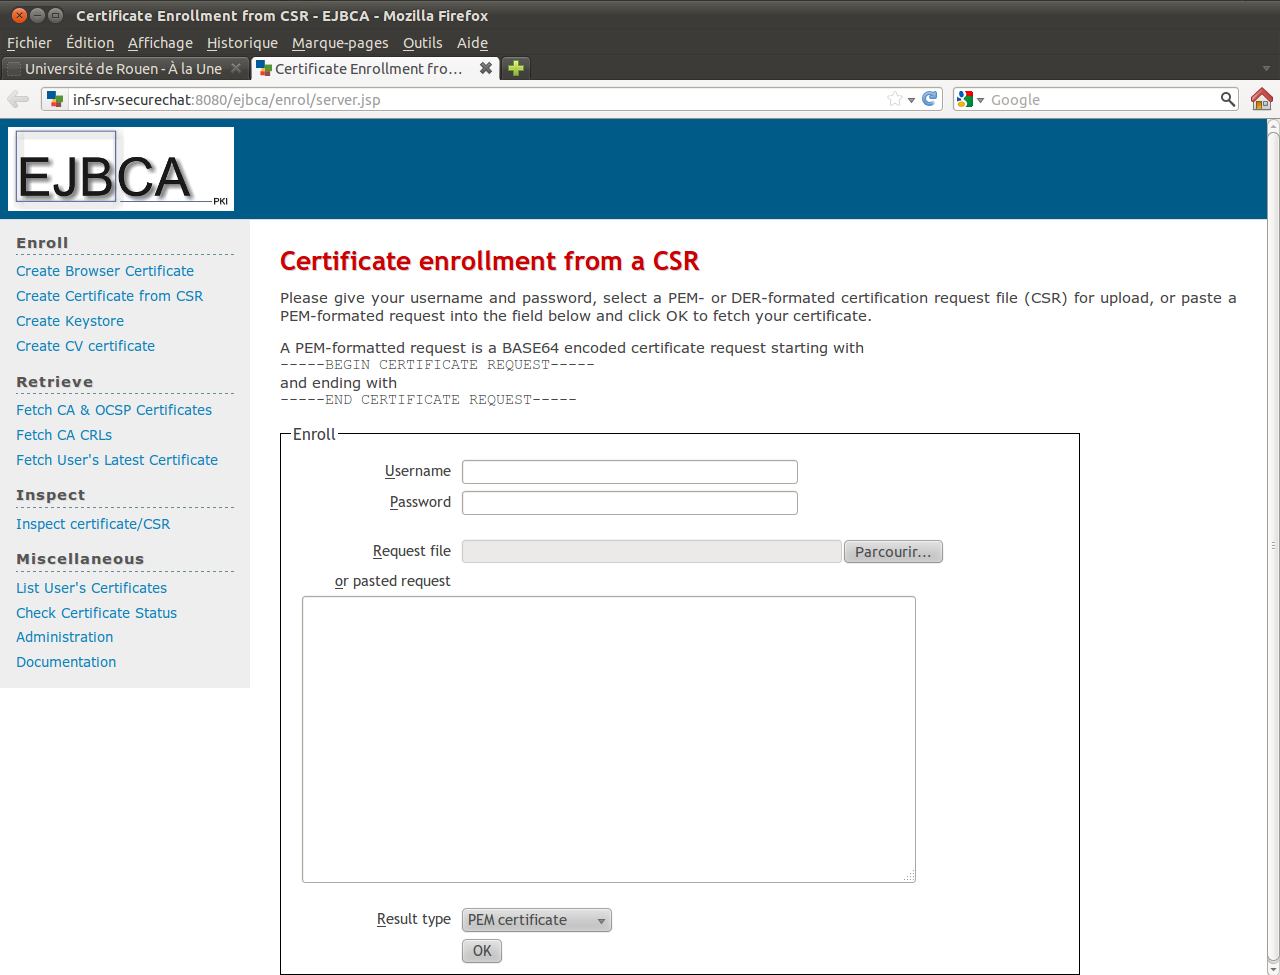
\includegraphics[scale=0.35]{capture/ejbca_cert.png}
\subsection{Serveur non sécurisé}
Pour lancer le serveur non sécurisé, il faut d'abord se rendre dans le répertoire "server" du répertoire build et taper les instructions suivantes:

\begin{verbatim}
    $ ./server ADRESSE_SERVEUR PORT_SERVEUR
\end{verbatim}

\verb+ADRESSE_SERVEUR+: l'adresse IP ou le nom de domaine du serveur non sécurisé

\verb+PORT_SERVEUR:+ le numéro du port d'écoute du serveur

\subsection{Serveur sécurisé}
Pour lancer le serveur sécurisé, il faut d'abord se rendre dans le répertoire "serversec" du répertoire "build" et taper les instructions suivantes:
\begin{verbatim}
    $ ./serversec ADRESSE_SERVEUR_SEC PORT_SERVEUR_SEC
\end{verbatim}

\verb+ADRESSE_SERVEUR_SEC+: l'adresse IP ou le nom de domaine du serveur sécurisé

\verb+PORT_SERVEUR_SEC+: le numéro du port d'écoute du serveur sécurisé
\\
\vspace{1.4cm}

\textbf{Contraintes:}\\ Le certificat client obtenu lors de la demande devra être placé dans le dossier client dont le chemin est: src/build/client.\\
Le certificat server devra être placé dans le dossier server\_sec dont le chemin est: src/build/server\_sec.\\
Le certificat racine root.pem devra être placé à la fois dans le dossier client et dans le dossier server\_sec.

\subsection{Client}
Pour lancer le client, il faut se rendre dans le répertoire "client" du répertoire "build" et lancer les instrutions suivantes:
\begin{itemize}
\item Client console : 
\begin{verbatim}
    $ ./clientsec-cli ADRESSE_SERVEUR PORT_SERVEUR ADRESSE_SERVEUR_SEC 
        PORT_SERVEUR_SEC CERTIFICAT CLE_PRIVEE [MOT_DE_PASSE_CLE] 
\end{verbatim}
\item Client Graphique :
\begin{verbatim}
    $ ./Client
\end{verbatim}
\end{itemize}

\verb+ADRESSE_SERVEUR+: l'adresse IP ou le nom de domaine du serveur non sécurisé.

\verb+PORT_SERVEUR+: le numéro du port d'écoute du serveur.

\verb+ADRESSE_SERVEUR_SEC+: l'adresse IP ou le nom de domaine du serveur sécurisé.

\verb+PORT_SERVEUR_SEC+: le numéro du port d'écoute du serveur sécurisé.

\verb+CERTIFICAT+: le chemin d'accès au certificat délivré par l'autorité de certification.

\verb+CLE_PRIVE+: la clé privée générée par l'utilisateur

\verb+MOT_DE_PASSE_CLE+: le mot de passe de la clé privée si elle a été généré avec un mot de passe.

	
\subsection{Utilisation du client console}
	
	La forme générale des commandes est : 
	
\verb+ /NOM_COMMANDE [paramètre_1 [Paramètre_2 [Paramètre_3 Paramètre_4]]]+

La commande de base de l'application est /HELP. Elle permet de lister toutes les commandes de l'application.
\subsubsection{Commandes du client classique et les actions}

\verb+	/CREATE_ROOM room_name+  : Permet de créer un salon ayant le nom "room\_name"

\verb+	/DELETE_ROOM room_name+ :  Permet de supprimer le salon du nom de "room\_name"

\verb+	/QUIT_ROOM room_name+ :  Permet de quitter le salon du nom de "room\_name"

\verb+	/JOIN_ROOM room_name+:  Rejoindre un salon du nom de "room\_name"

\verb+	/DISCONNECT+: Se déconnecter du serveur non sécurisé

\verb+	/CONNECT user+:  Se connecter avec l'identifiant "user"

\verb+	/MP user message+: Envoyer un message privé à l'utilisateur "user"
			
\subsubsection{Commandes du client sécurisé et les actions}

\verb+	/CONNECT_SEC user user_certif user_key+: Connexion au serveur sécurisé avec le nom d'utilisateur "user" avec le certificat "user\_certif" et la clé privée "user\_key" (Si la clé privée a été créée avec un mot de passe, il faut ajouter le mot de passe après "user\_key")

\verb+	/CREATE_ROOM_SEC room_name+: Permet de créer un salon sécurisé du nom de "room\_name"

\verb+	/DELETE_ROOM_SEC room_name+: Permet de supprimer le salon sécurisé du nom "room\_name"

\verb+	/DISCONNECT_SEC+: Se déconnecter du serveur sécurisé et du serveur non sécurisé

\verb+	/QUIT_ROOM_SEC room_name+: Quitter le salon sécurisé du nom de "room\_name"

\verb+	/JOIN_ROOM_SEC room_name+: Rejoindre le salon sécurisé du nom de "room\_name"

\verb+	/DEL_ACCOUNT_SEC+: Supprimer le compte utilisateur sécurisé

\verb+	/MP_SEC user message+: Envoyer un message privé sécurisé

\verb+	/MESSAGE room_name message+: Envoyer le message "message" sur le salon "room\_name"

\verb+	/ACCEPT_JOIN_ROOM_SEC room_name user+: Accepter l'ajout d'un utilisateur qui fait la demande pour rejoindre le salon "room\_name". Seul l'administrateur du salon a les droits pour effectuer cette opération.

\verb+	/REFUSE_JOIN_ROOM_SEC room_name user+: Refuser la requête d'ajout qu'un utilisateur a envoyé pour rejoindre un salon. Seul l'administrateur du salon a les droits pour effectuer cette opération.

\verb+	/EJECT_FROM_ROOM_SEC room_name user+: Supprimer un utilisateur "user" du salon "room\_name". Seul l'administrateur du salon a les droits pour effectuer cette opération.


\subsection{Utilisation du client graphique}

Le client graphique permet d'effectuer les mêmes opérations que le client console mais avec l'intuitivité que nous offre l'interface graphique.

\subsubsection{Connexion non sécurisée}
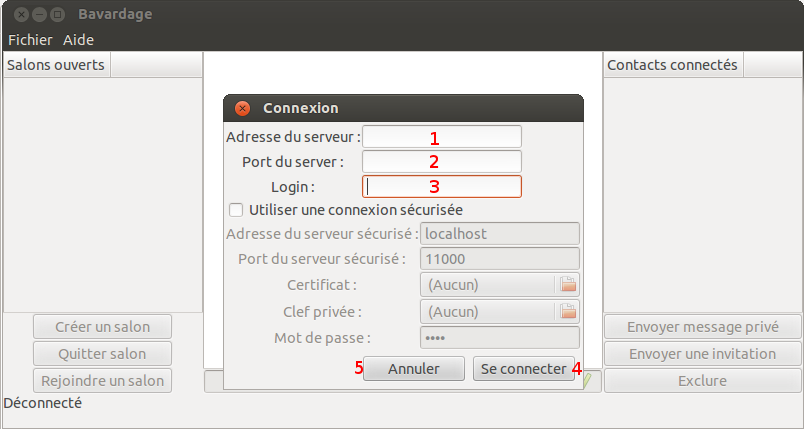
\includegraphics[width=40em]{capture/con_n_sec.png}

Pour effectuer une connexion non sécurisée, il faut:
\begin{enumerate}
    \item Entrer l'adresse du serveur non sécurisé;
    \item Entrer le port d'écoute du serveur non sécurisé;
    \item Entrer le login voulu pour se connecter;
    \item Cliquer sur le bouton "Se connecter" pour lancer la connexion;
    \item Cliquer sur le bouton "Annuler" pour annuler la connexion;
\end{enumerate}

\subsubsection{Connexion sécurisée}

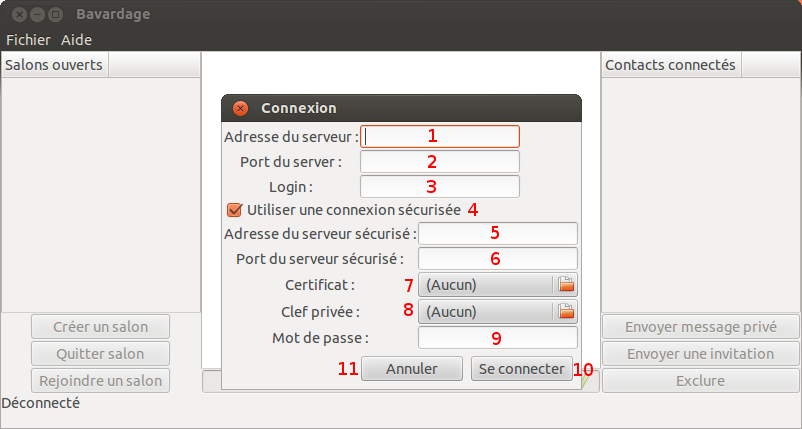
\includegraphics[width=40em]{capture/con_sec.png}

Pour effectuer une connexion sécurisée, il faut:

\begin{enumerate}
    \item Entrer l'adresse du serveur non sécurisé;
    \item Entrer le port d'écoute du serveur non sécurisé;
    \item Entrer le login voulu pour se connecter;
    \item Cocher l'option de connexion sécurisée;
    \item Entrer l'adresse du serveur sécurisé;
    \item Entrer le port d'écoute du serveur sécurisé;
    \item Sélectionner le fichier du certificat délivré par l'autorité de certification;
    \item Sélectionner le fichier de la clé privée;
    \item Entrer le mot de passe correspondant à la clé privée (Si aucun mot de passe n'a été utilisé pour générer la clé privée, ne rien entrer dans ce champ);
    \item Cliquer sur le bouton "Se connecter" pour lancer la connexion;
    \item Cliquer sur le bouton "Annuler" pour annuler la connexion;
\end{enumerate}
\newpage

\subsubsection{Création d'un salon (sécurisé ou non sécurisé)}

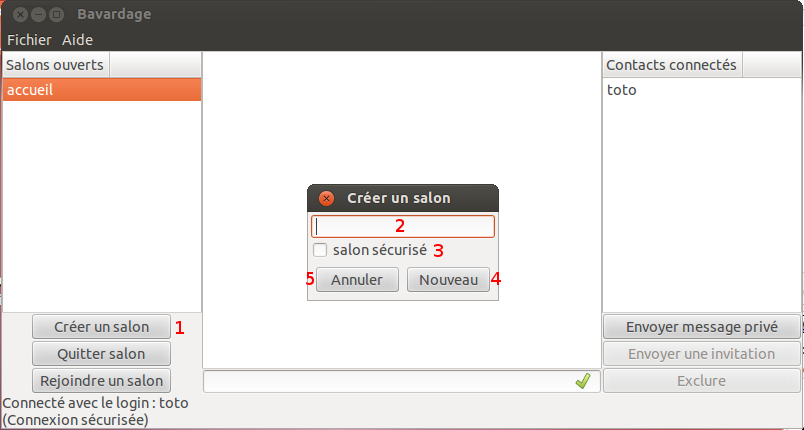
\includegraphics[width=40em]{capture/cre_room.png}

Pour effectuer la création d'un salon (sécurisé ou non sécurisé), il faut:
\begin{enumerate}
    \item Cliquer sur le bouton "Créer un salon";
    \item Entrer le nom du salon à créer dans le champ;
    \item Cocher le champ "salon sécurisé" s'il s'agit d'un salon sécurisé;
    \item Cliquer sur le bouton "Nouveau" pour créer le salon;
    \item Cliquer sur le bouton "Annuler" pour annuler la création du salon.
\end{enumerate}
\newpage

\subsubsection{Rejoindre un salon (sécurisé ou non sécurisé)}

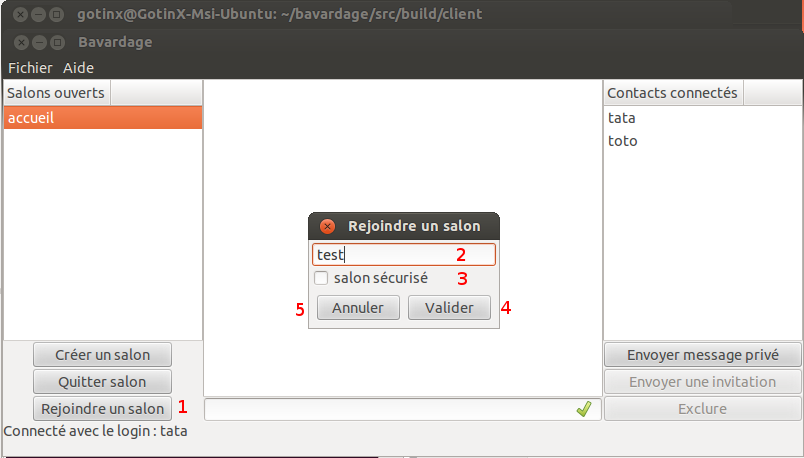
\includegraphics[width=40em]{capture/rej_sal.png}

Pour rejoindre un salon (sécurisé ou non sécurisé), il faut:

\begin{enumerate}
    \item Cliquer sur le bouton rejoindre un salon;
    \item Entrer le nom du salon à rejoindre;
    \item Cocher la case "salon sécurisé";
    \item Cliquer sur le bouton "Se connecter" pour rejoindre le salon s'il n'est pas sécurisé ou envoyer une demande à l'administrateur du salon si le salon est sécurisé;
    \item Cliquer sur le bouton "Annuler" pour annuler la connexion.
\end{enumerate}
\newpage

\subsubsection{Envoyer un message dans un salon}

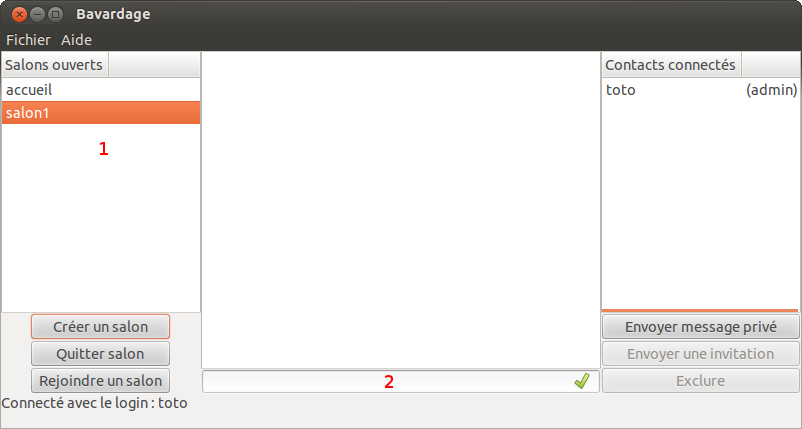
\includegraphics[width=40em]{capture/mess_room.png}

Pour envoyer un message dans un salon, il faut:
\begin{enumerate}
    \item Sélectionner le salon dans lequel on veut envoyer le message dans la liste des salons ouverts;
    \item Saisir le message dans la zone puis appuyer sur la touche "Entrée" pour envoyer le message.
\end{enumerate}

\subsubsection{Envoyer un message privé à un utilisateur}

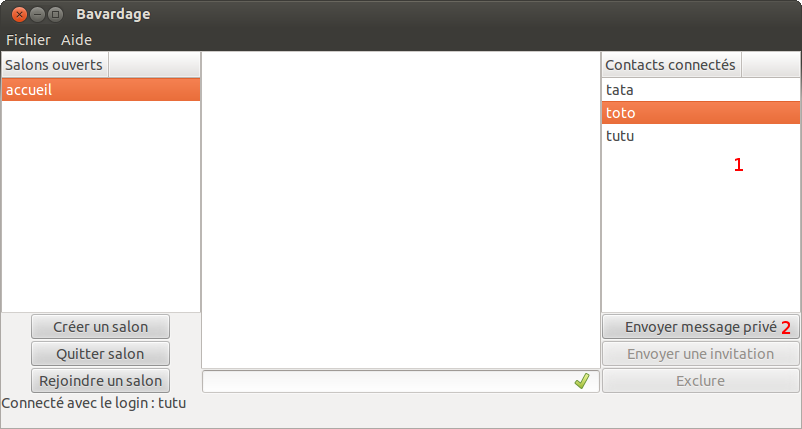
\includegraphics[width=40em]{capture/mp_nsec.png}

Pour envoyer des messages en mode privé à un utilisateur, il faut:

\begin{enumerate}
    \item Sélectionner l'utilisateur dans la liste des contacts connectés;
    \item Cliquer sur le bouton "Envoyer message privé".
    \item Une boite de dialogue s'afficher pour demander si l'on veut une discussion sécurisée avec l'utilisateur 
\end{enumerate}

\subsubsection{Accepter la requête d'un utilisateur qui souhaite rejoindre un salon}

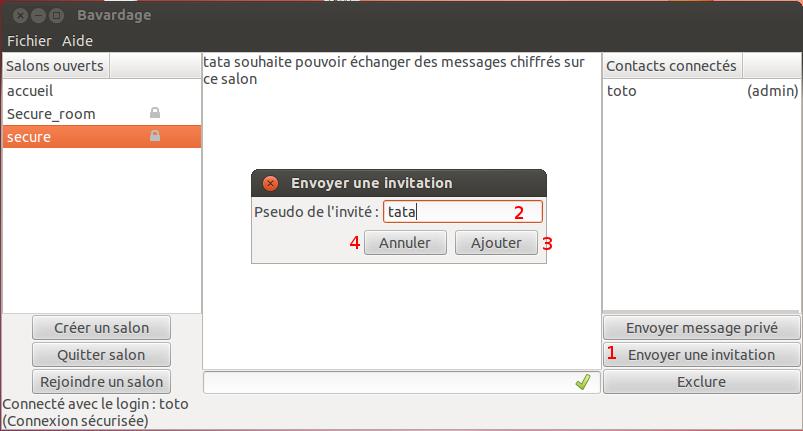
\includegraphics[width=40em]{capture/invit_room.png}

Pour accepter une demande d'invitation reçu,
\begin{enumerate}
    \item Cliquer le bouton "Envoyer une invitation";
    \item Entrer le pseudo de l'utilisateur ayant envoyé la demande;
    \item Cliquer le bouton "Ajouter" pour rajouter l'utilisateur au salon sécurisé
    \item Cliquer sur le bouton "Annuler" pour annuler l'ajout de l'utilisateur
\end{enumerate}

\subsubsection{Exclure un utilisateur}
Pour exclure un utilisateur,
\begin{enumerate}
    \item Sélectionner le pseudo de l'utilisateur dans la liste des contacts connectés;
    \item Cliquer sur "Exclure".
\end{enumerate}
\newpage

\subsubsection{Quitter un salon}

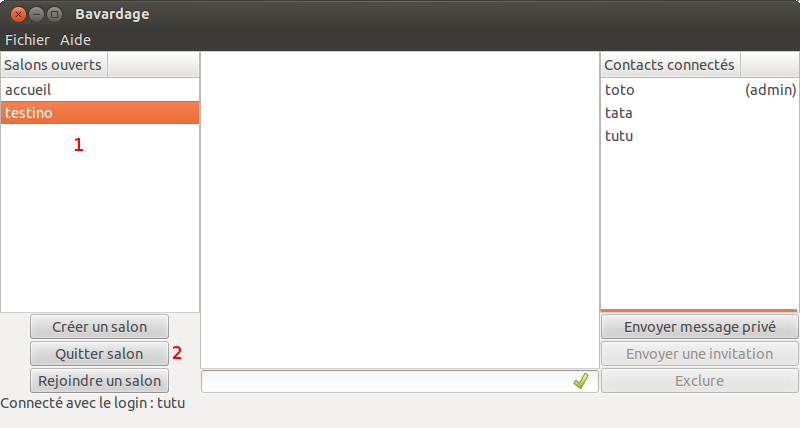
\includegraphics[width=40em]{capture/quit_room.png}

Pour quitter un salon, il faut:

\begin{enumerate}
    \item Sélectionner le salon que l'on veut quitter dans la liste des salons ouverts;
    \item Cliquer sur le bouton "Quitter salon".

\end{enumerate}

\subsubsection{Se déconnecter}
Pour se déconnecter,
\begin{enumerate}
    \item Aller dans le menu "Fichier";
    \item Cliquer sur "Déconnecter".
\end{enumerate}

\newpage
%%%%%%%%%%%%%%%%%%%%%%%%%%%%%%%%%%%%%%%%%%%%
% CONCLUSION 
% JB
%%%%%%%%%%%%%%%%%%%%%%%%%%%%%%%%%%%%%%%%%%%%
\large
\chapter{Conclusion}

Ce projet a été découpé en deux parties distinctes, l'analyse et l'étude d'un sujet associées à une gestion de projet
afin de proposer une solution au client puis une deuxième phase qui a été 
l'implémentation de la solution proposée également accompagnée d'une gestion de 
projet.\\

L'étude et l'analyse théorique du sujet lors de la première phase de projet nous a permis
d'apprendre à mettre en place des documents spécifiques et détaillés sur chaque fonctionnalités en utilisant des méthodes de conception 
professionnelle. La méthode agile scrum que nous avons choisie a permis d'établir un planning de gestion et un découpage astucieux du projet en plusieurs
étapes et ainsi proposer une solution structurée respectant au mieux les besoins du client.\\

La deuxième phase d'implémentation a été un moyen de mettre en pratique 
nos techniques de programmation acquises au cours de nos formations antérieures, nos connaissances théoriques en cryptographie
mais également d'apprendre de nouvelles technologies, en particulier pour la mise en place des techniques de cryptographie 
et la gestion d'une autorité de certification avec certificats dans une application concrète et fonctionnelle.\\

La méthode agile scrum utilisée pour ce projet a simplifié les phases afin d’en raccourcir la durée.
Les méthodes agiles, se basent sur la notion de communauté de projet dans laquelle les développeurs
et les utilisateurs sont présents en permanence pour exprimer ou répondre à une question liée au projet. 
C'est une communication permanente entre les membres du groupe de projet, et le client qui a fait que 
nous avons su rapidement prendre en compte les opinions et idées de chacun et de réagir aux 
différents problèmes que ce soit lors de l'analyse ou de l'implémentation du 
projet. Nous en tirons donc une expérience très enrichissante sur la gestion et 
la communication au sein d'un groupe de projet dans un cadre orienté professionnel.



\newpage
\appendix
\chapter{Documents de gestion de projet}
\begin{itemize}
\item Spécification technique des besoins : \url{https://github.com/legrajul/bavardage-doc/raw/master/STB/stb.pdf};
\item Document d'architecture logicielle : \url{https://github.com/legrajul/bavardage-doc/raw/master/DAL/dal.pdf};
\item Analyse des risques : \url{https://github.com/legrajul/bavardage-doc/raw/master/ADR/adr.pdf};
\item Cahier de recette : \url{https://github.com/legrajul/bavardage-doc/raw/master/CdR/cdr.pdf}\\
\url{https://github.com/legrajul/bavardage-doc/raw/master/CdR/CdR.xlsx};
\item Plan de développement : \url{https://github.com/legrajul/bavardage-doc/raw/master/PDD/pdd.pdf};
\end{itemize}
\chapter{Déclaration des pratiques de certification}
\url{https://github.com/legrajul/bavardage-doc/raw/master/DPC/dpc.pdf}
\chapter{Politique de certification}
\url{https://github.com/legrajul/bavardage-doc/raw/master/PC/pc.pdf}
\end{document}